% Theory of Code Space (ToCS) — v0.1 Concept Paper
\documentclass{article}

\usepackage[preprint]{neurips_2025}

\usepackage[utf8]{inputenc}
\usepackage[T1]{fontenc}
\usepackage{hyperref}
\usepackage{url}
\usepackage{booktabs}
\usepackage{amsfonts}
\usepackage{amsmath}
\usepackage{amssymb}
\usepackage{graphicx}
\usepackage{xcolor}
\usepackage{subcaption}
\usepackage{multirow}
\usepackage{makecell}
\usepackage{enumitem}

\newcommand{\tocs}{\textsc{ToCS}}
\newcommand{\tos}{\textsc{ToS}}
\newcommand{\pms}[1]{\,{\scriptsize$\pm$\,#1}}

\title{Theory of Code Space: Do Code Agents Understand Software Architecture?}

\author{
  Grigory Sapunov\thanks{Work in progress. LLM results are preliminary (single run per model-codebase pair); subsequent versions will include repeated runs with variance estimation, additional models, and codebase patterns. Collaborations welcome.} \\
  Intento \\
  \texttt{gs@inten.to}
}

\begin{document}

\maketitle

% ============================================================================
\begin{abstract}
AI code agents excel at isolated tasks---writing functions, fixing localized bugs---yet struggle with complex, multi-file software engineering that requires understanding how dozens of modules relate to each other. We hypothesize that these failures stem from an inability to construct, maintain, and update coherent \emph{architectural beliefs} during codebase exploration. We introduce \textbf{Theory of Code Space} (\tocs{}), a benchmark that evaluates this capability by placing agents in procedurally generated codebases under partial observability, requiring them to build structured belief states over module dependencies, cross-cutting invariants, and design intent. Our framework makes three key design choices: (1)~a procedural codebase generator producing medium-complexity Python projects with four typed edge categories reflecting different discovery methods---from syntactic imports to config-driven dynamic wiring---with planted architectural constraints and verified ground truth; (2)~a partial observability harness where agents explore under a budget, ensuring that exploration strategy matters; and (3)~periodic belief probing via structured JSON, producing a time-series of architectural understanding rather than a single final snapshot. We decompose the Active-Passive Gap from spatial reasoning benchmarks into selection and decision components, and introduce Architectural Constraint Discovery as a code-specific evaluation dimension absent from spatial domains. Preliminary experiments with four rule-based baselines and six frontier LLM agents from three providers validate the benchmark's discriminative power: methods span a wide performance range (Dependency F1 from 0.147 to 0.676), LLM agents discover semantic edge types invisible to all baselines and achieve non-trivial architectural invariant discovery (relaxed F1 up to 0.78), yet weaker models score below simple heuristics---revealing that \emph{belief externalization} and \emph{belief state maintenance} are themselves non-trivial capabilities: some models catastrophically forget previously-discovered components between probes, with the surprising result that a smaller model (Gemini~2.5~Flash) maintains perfectly stable beliefs while its larger sibling (Gemini~2.5~Pro) suffers catastrophic belief collapse. We release the complete toolkit as open-source software and invite the community to evaluate additional models and contribute codebase patterns.\footnote{Code: \url{https://github.com/che-shr-cat/tocs}}
\end{abstract}

% ============================================================================
\section{Introduction}
\label{sec:intro}

Large language models achieve remarkable scores on code generation benchmarks~\citep{chen2021codex, austin2021program}, creating an expectation that they possess deep understanding of software architecture. Yet practitioners report a persistent gap: models that solve HumanEval problems with ease produce incoherent results when modifying real codebases with dozens of interdependent modules~\citep{jimenez2024swebench}. This gap has resisted satisfying explanation.

Recent work on spatial reasoning offers a compelling diagnostic framework. \citet{zhang2026theoryofspace} introduced the \emph{Theory of Space} (\tos{}) benchmark, demonstrating that multimodal models fail to maintain coherent internal ``cognitive maps'' when actively exploring partially observable environments. They identified two core phenomena: an \textbf{Active-Passive Gap} (models degrade when they must gather information themselves rather than receiving it upfront) and \textbf{Belief Inertia} (models cannot update their spatial beliefs when the environment changes). We hypothesize that the same latent state maintenance failures explain the struggles of code agents. The term ``cognitive map'' traces to \citet{tolman1948cognitive}; in program comprehension, \citet{pennington1987stimulus} and \citet{vonmayrhauser1995program} showed that developers build layered mental models of code---our benchmark operationalizes and measures this process for AI agents.

We propose \textbf{Theory of Code Space} (\tocs{}), a benchmark that transplants this diagnostic framework to software engineering. Rather than grid worlds, our ``environment'' consists of procedurally generated codebases with controlled architectural structure. Rather than allocentric spatial maps, our ``cognitive maps'' are structured representations of module dependencies, typed edges, cross-cutting invariants, and design intent. The agent explores under partial observability---opening files one at a time under a budget---and must externalize its architectural belief as structured JSON at regular intervals.

Beyond the spatial analogy, we introduce \textbf{Architectural Constraint Discovery}---a dimension absent from spatial benchmarks. In code, architectural decisions encode \emph{checkable constraints}: a forbidden dependency enforces a service boundary; a validation chain ensures data integrity. We plant explicit, verifiable constraints in our generated codebases and measure whether agents can discover them.

Our contributions are:
\begin{enumerate}[nosep]
    \item The \tocs{} benchmark framework: the first evaluation for active architectural belief construction, revision, and exploitation in code (\S\ref{sec:benchmark}).
    \item A procedural codebase generator producing medium-complexity projects with four typed edge categories, planted invariants, and verified ground truth (\S\ref{sec:generation}).
    \item Pilot experiments with four baselines and four frontier LLM agents from three providers, showing that the two strongest agents surpass all baselines (F1~=~0.676 and 0.650 vs.\ 0.577) while revealing a wide capability spread: LLM agents discover all four edge types and, under improved prompts, achieve non-trivial invariant discovery (relaxed F1 up to 0.78), yet weaker models score below simple heuristics (\S\ref{sec:results}).
    \item An open benchmark with evaluation harness, scoring pipeline, and community call for expanded model evaluation (\S\ref{sec:discussion}).
\end{enumerate}

% ============================================================================
\section{Related Work}
\label{sec:related}

\paragraph{Code Generation Benchmarks.}
SWE-bench~\citep{jimenez2024swebench} evaluates bug-fixing in real GitHub repositories but measures patch correctness, not evolving architectural understanding. ContextBench~\citep{li2026contextbench} advances this by logging agent trajectories and scoring context retrieval precision/recall against human-verified gold contexts---measuring \emph{what the agent looked at} but not \emph{what the agent believes about architecture}. SWE-ContextBench~\citep{zhu2026swecontextbench} tests cross-task experience reuse. RepoBench~\citep{liu2024repobench} and LoCoBench-Agent~\citep{qiu2025locobench} evaluate repo-level completion and long-context interaction respectively, with LoCoBench observing a ``comprehension-efficiency trade-off'' that we formalize as the Active-Passive Gap. RefactorBench~\citep{masai2025refactorbench} targets multi-file refactoring but evaluates output correctness without probing belief state. None of these benchmarks require agents to \emph{externalize} a revisable architectural belief state, impose exploration budgets, or score against typed dependency graphs with planted constraints. We note that our own belief externalization finding (\S\ref{sec:results}) reveals a complementary limitation: even when agents \emph{do} externalize beliefs, what they report may not reflect what they internally represent.

\paragraph{Code Understanding Tools.}
CodePlan~\citep{bairi2024codeplan} augments LLMs with static-analysis dependency graphs for change propagation---an engineering solution that validates our premise: agents need architectural maps but currently cannot build them alone. Aider's RepoMap~\citep{gauthier2024aider} uses tree-sitter parsing and PageRank to construct repository context. Code World Models~\citep{fair2025cwm} train LLMs on execution traces to improve code reasoning. \tocs{} provides the diagnostic benchmark to test whether such approaches actually improve architectural belief quality.

\paragraph{Spatial Reasoning.}
Theory of Space~\citep{zhang2026theoryofspace} demonstrated Active-Passive Gap and Belief Inertia in grid-world environments with multimodal models. Related spatial benchmarks include SpatialVLM~\citep{spatialvlm2024}, Habitat~\citep{habitat2019}, and OpenEQA~\citep{openeqa2024}, which evaluate spatial reasoning and embodied question answering but do not require constructing revisable belief states. We transplant this framework to code, adding architectural constraint discovery (absent from spatial domains where object placement ``why'' is rarely meaningful). TOM-SWE~\citep{zhou2025tomswe} models the \emph{user's} mental state in SWE agents---complementary to our focus on the agent's belief about the \emph{codebase}.

% ============================================================================
\section{Theory of Code Space}
\label{sec:benchmark}

\subsection{Problem Formulation}

We formalize codebase understanding as \emph{belief construction} over a latent architectural state. Let $S$ denote the ground-truth architecture, comprising a typed dependency graph $G = (V, E)$ with edge types $\tau \in \{\textsc{imports}, \textsc{calls\_api}, \textsc{data\_flows\_to}, \textsc{registry\_wires}\}$, a set of cross-module invariants $\mathcal{I}$, and exported contracts $\mathcal{C}$. At time $t$, the agent has history $h_t = (o_{0:t}, a_{0:t})$ and we evaluate three operations on its belief $\mathcal{M}_t(S)$.  Since $\mathcal{M}_t$ is a latent internal state, we measure it through \emph{probing}: periodically asking the agent to externalize its belief as structured JSON (\S\ref{sec:probing}). We evaluate:

\begin{description}[nosep]
    \item[Construct] Build $\mathcal{M}_t$ from partial observations gathered through active exploration.
    \item[Revise] Update $\mathcal{M}_t \to \mathcal{M}_{t+\Delta t}$ when the environment mutates ($S \to S'$) and the agent encounters evidence of the change.
    \item[Exploit] Use $\mathcal{M}_t$ to perform a downstream engineering task correctly (v1.0; v0.1 uses counterfactual probes as a proxy).
\end{description}

\subsection{Environment and Action Space}

The agent interacts with the codebase through five actions with \textbf{fixed tool semantics}:
\begin{itemize}[nosep]
    \item \texttt{LIST}($d$): Filenames in directory $d$ (no contents, no recursion).
    \item \texttt{OPEN}($f$): Full contents of file $f$. Costs 1 action.
    \item \texttt{SEARCH}($q$): Matching filepaths + line numbers. \textbf{No content snippets.} Costs 1 action.
    \item \texttt{INSPECT}($f$, $s$): Type signature + docstring of symbol $s$. No body. Costs 1 action.
    \item \texttt{DONE}(): Terminate. Costs 0 actions.
\end{itemize}
The agent operates under a budget $B$ (default $B{=}20$). Critically, \texttt{SEARCH} returns only locations, never content---ensuring that architectural understanding requires deliberate \texttt{OPEN} decisions. \texttt{INSPECT} provides a lightweight discovery channel: docstrings often describe module purpose and relationships (e.g., ``wraps stage X''), allowing agents to gather architectural hints at the cost of one action without reading full file contents.

\subsection{Cognitive Map Probing}
\label{sec:probing}

Every $K{=}3$ actions, the harness interrupts the agent with a structured prompt requesting it to externalize its current architectural belief as JSON. Critically, \textbf{probing is free}: it does not consume an action from the budget $B$, and the agent retains the same remaining budget before and after a probe. This ensures that measurement does not interfere with exploration strategy---agents are evaluated on their understanding, not on a trade-off between exploring and reporting.

The externalized cognitive map $\hat{\mathcal{M}}_t$ contains: (1) \textbf{component beliefs} with status (observed/inferred/unknown), purpose, exported symbols with typed signatures, and typed dependency edges with per-element confidence; (2) \textbf{invariant beliefs} with structured canonical form (\texttt{type, src, dst, via, pattern}) and evidence pointers; (3) \textbf{uncertainty tracking}---explicit list of unexplored regions. The resulting time-series of maps (one every $K$ steps) captures \emph{how} understanding develops, not just the final state.

\subsection{Evaluation Modes}

\tocs{} decomposes the Active-Passive Gap through four conditions:
\begin{itemize}[nosep]
    \item \textbf{Active}: Agent chooses actions under budget $B$.
    \item \textbf{Passive-Full}: Agent receives the entire codebase; probed once.
    \item \textbf{Passive-Oracle}: Agent receives $B$ files selected by oracle (maximum ground-truth connectivity); one file per step, probed every $K$.
    \item \textbf{Passive-Replay}: Agent receives the \emph{exact observation trace} from a prior active run, without making decisions. Each observation counts as one step.
\end{itemize}

This decomposes: $\text{APG}_\text{total}$ (passive-full $-$ active) into $\text{APG}_\text{selection}$ (passive-oracle $-$ active, the cost of choosing \emph{which} files) and $\text{APG}_\text{decision}$ (passive-replay $-$ active, the cost of deciding \emph{what to do} with observations).

\noindent\textbf{Scope note:} v0.1 evaluates the \textbf{Construct} operation in \textbf{Active} mode only. The passive conditions and APG decomposition are implemented in the harness and reserved for future work with frontier model evaluations.

\subsection{Architectural Constraint Discovery}

Beyond structural mapping, we probe whether agents discover planted architectural constraints:
\begin{itemize}[nosep]
    \item \textbf{Forbidden dependency}: ``Module $A$ must not import module $C$ directly.''
    \item \textbf{Interface-only access}: ``Module $X$ must access $Y$ only through interface $Z$.''
    \item \textbf{Validation chain}: ``Data must pass through validation before reaching module $W$.''
\end{itemize}
Each constraint has a \textbf{discoverability requirement}: test evidence, structural patterns, or documentation in the codebase. Scored via counterfactual multiple-choice probes (``Which change would violate an architectural constraint?'').

% ============================================================================
\section{Procedural Codebase Generation}
\label{sec:generation}

\subsection{Architecture Grammar}

Our v0.1 generator produces \textbf{Pipeline} architecture codebases with controlled anti-triviality measures. A \texttt{PipelineTemplate} grammar defines:

\begin{itemize}[nosep]
    \item \textbf{Domain pools}: Three domains (data ETL, log processing, text processing), each with 8 semantically coherent processing stages. Medium complexity selects 6--8 stages.
    \item \textbf{Module roles}: Infrastructure (models, base class, config, exceptions, registry), stages (processing steps implementing a common ABC), adapters (wrapping stages with additional behavior), middleware (cross-cutting decorators), utilities, and legacy/distractor modules.
    \item \textbf{Anti-triviality}: (1) \emph{Registry wiring}---stages connected via config, not direct imports; (2) \emph{Adapter indirection}---ABC interface layer; (3) \emph{Distractor modules}---files not in the main pipeline; (4) \emph{Neutral naming}---\texttt{mod\_a.py}, not \texttt{extract.py}; (5) \emph{Hidden invariants}---constraints discoverable only by reading function bodies or tests.
\end{itemize}

\subsection{Four Edge Types}

Each generated codebase contains edges of four types, reflecting different \emph{methods of discovery}:
\begin{itemize}[nosep]
    \item \textsc{imports} ($\sim$67\%): Python \texttt{import} statements. Discoverable by AST parsing.
    \item \textsc{calls\_api} ($\sim$17\%): Runtime function calls between modules. Requires reading function bodies; docstrings may provide hints (e.g., ``delegates to module X'').
    \item \textsc{registry\_wires} ($\sim$9\%): Config-driven connections where a registry module dynamically loads stages via \texttt{importlib} based on names listed in a JSON config file. No static \texttt{import} statement exists. Requires reading both the config and the registry's loading logic.
    \item \textsc{data\_flows\_to} ($\sim$7\%): Data dependency where one module's output feeds another's input. Requires understanding orchestration logic; docstrings on the orchestrator may describe the data flow.
\end{itemize}

These proportions are not tunable parameters but \emph{emerge from the architectural template}: a Pipeline with $N$ stages naturally generates $\sim$3--4$\times$ more \textsc{imports} edges because every module requires static imports, while semantic edge types arise only at specific architectural boundaries (adapter$\to$stage, orchestrator$\to$stage, consecutive stages). This mirrors real-world Pipeline codebases, where import edges dominate. Different architectural patterns (event-driven, microservices) would yield different distributions---a key motivation for extending the generator. Crucially, roughly one-third of edges are \emph{invisible to import-following} (specific to our Pipeline template; other architectural patterns would yield different proportions), creating a meaningful gap between syntactic analysis and semantic understanding.

\subsection{Invariant Planting}

Each codebase contains 15--16 planted constraints across five types: \textsc{boundary} (forbidden dependencies), \textsc{dataflow} (required processing chains), \textsc{interface} (access-only-through-ABC), \textsc{invariant} (naming/structural conventions), and \textsc{purpose} (design rationales). Every constraint has a \emph{structured canonical form} with five fields for machine-comparable scoring: \texttt{type} (constraint category), \texttt{src} and \texttt{dst} (the modules involved), \texttt{via} (the intermediary or mechanism, e.g., an ABC interface), and \texttt{pattern} (the structural rule, e.g., ``no direct import''). For example, a boundary constraint might be \texttt{(boundary, mod\_a, mod\_c, base.StageBase, ``must access only through ABC'')}. Each constraint has at least one evidence source (test file, structural pattern, or documentation).

\subsection{Generation Statistics}

\begin{table}[!ht]
\centering
\caption{Generated codebase characteristics (medium complexity, 3 seeds).}
\label{tab:codebases}
\begin{tabular}{@{}lccc@{}}
\toprule
\textbf{Metric} & \textbf{Seed 42} & \textbf{Seed 123} & \textbf{Seed 999} \\
\midrule
Modules & 27 & 30 & 27 \\
Total edges & 70 & 84 & 70 \\
\quad \textsc{imports} & 47 (67\%) & 56 (67\%) & 47 (67\%) \\
\quad \textsc{calls\_api} & 12 (17\%) & 15 (18\%) & 12 (17\%) \\
\quad \textsc{data\_flows\_to} & 5 (7\%) & 6 (7\%) & 5 (7\%) \\
\quad \textsc{registry\_wires} & 6 (9\%) & 7 (8\%) & 6 (9\%) \\
Invariants & 15 & 16 & 15 \\
Sub-packages & 5 & 5 & 5 \\
\bottomrule
\end{tabular}
\end{table}

% ============================================================================
\section{Metrics}
\label{sec:metrics}

\paragraph{Dependency F1.}
Compare predicted edges from the cognitive map against ground truth. An edge matches if (source, target, type) all agree via exact string matching. Targets must be specific file paths: a directory-level edge (e.g., \texttt{registry.py $\to$ stages/}) does not match file-level ground truth (e.g., \texttt{registry.py $\to$ stages/mod\_a.py}). Similarly, symbol-qualified targets (e.g., \texttt{base.py::StageBase} instead of \texttt{base.py}) do not match even when the file path portion is correct. This strict matching is deliberate---our ground truth is component-level (one file = one node)---but means that models reporting correct relationships at the wrong granularity or format receive no credit. We report precision, recall, and F1 separately.

\paragraph{Invariant F1.}
Match agent-discovered constraints against planted constraints via \emph{structured form} comparison---exact field matching on \texttt{(type, src, dst, via)}, not text similarity. This eliminates ambiguity in natural-language descriptions.

\paragraph{Confidence Calibration.}
Expected Calibration Error (ECE) between agent-stated per-edge confidence and actual correctness, binned into 5 confidence intervals.

\paragraph{Two Efficiency Curves.}
\emph{Action-efficiency}: AUC(F1 vs.\ total actions)---the headline metric. \emph{Observation-efficiency}: AUC(F1 vs.\ \texttt{OPEN} count)---diagnostic, isolating information gain per file opened. Belief is piecewise-constant between probes; integration is trapezoidal.

\paragraph{Active-Passive Gap.}
For each metric $m$: $\text{APG}_m = m_\text{passive} - m_\text{active}$, decomposed into selection and decision components as described in \S\ref{sec:benchmark}.

\paragraph{Belief Revision Score (BRS).}
After a mutation at time $t_m$: $\text{BRS} = |\text{correctly updated}| / |\text{affected elements}|$. Decomposed into \emph{Inertia-proper} (correctly-believed elements not updated after evidence) and \emph{Impact-discovery} (missing elements newly found). A \emph{sham condition} (evidence without actual change) measures Gullibility. (BRS evaluation is implemented but reserved for future work.)

% ============================================================================
\section{Experiments}
\label{sec:results}

We evaluate four rule-based exploration strategies and five frontier LLM agents from three providers on three generated codebases (seeds 42, 123, 999) under identical conditions: budget $B{=}20$, probe interval $K{=}3$. These results are preliminary; we report them to validate the benchmark's discriminative power and invite community replication.

\subsection{Methods}

\paragraph{Rule-based baselines.}
\begin{itemize}[nosep]
    \item \textbf{Oracle}: Outputs the ground-truth graph directly. Upper bound (F1 = 1.0).
    \item \textbf{Config-Aware}: Lists all directories, opens config/registry files first, parses module references, then follows imports BFS.
    \item \textbf{Random}: Lists root, then opens files uniformly at random until budget exhausted. Builds map from observed imports.
    \item \textbf{BFS-Import}: Opens files breadth-first following import chains.
\end{itemize}
All baselines build cognitive maps from AST-parsed imports and config references.

\paragraph{LLM agents.}
\begin{itemize}[nosep]
    \item \textbf{GPT-5.3-Codex}: OpenAI's code-specialized reasoning model (\texttt{gpt-5.3-codex}). A reasoning model (temperature fixed at 1 per API constraint).
    \item \textbf{Claude Sonnet 4.6}: Anthropic's frontier coding model (\texttt{claude-sonnet-4-6}).
    \item \textbf{Gemini 2.5 Flash}: Google's reasoning-optimized flash model (\texttt{gemini-2.5-flash}). A ``thinking'' model with extended internal reasoning.
    \item \textbf{Gemini 2.5 Pro}: Google's reasoning-optimized pro model (\texttt{gemini-2.5-pro}). Larger sibling of 2.5~Flash.
    \item \textbf{Gemini 3 Flash}: Google's frontier flash model (\texttt{gemini-3-flash-preview}).
    \item \textbf{Gemini 3.1 Pro}: Google's most capable model (\texttt{gemini-3.1-pro-preview}). The flagship of the Gemini~3 family.
\end{itemize}
All models receive identical prompts: a system prompt describing the partial observability environment and available actions, per-turn action prompts showing remaining budget and opened files, and structured JSON probe prompts with schema, per-type field semantics, and worked examples for each invariant type (Appendix~\ref{app:prompts}). Relative to an earlier prompt version, the current probe includes explicit edge type decision rules and pairwise invariant decomposition instructions. Temperature is set to 0 except for GPT-5.3-Codex (reasoning model constraint). All probe responses were parsed successfully via the deterministic repair parser (zero format failures across all runs).

\subsection{Results}

\begin{table}[!ht]
\centering
\caption{Performance over 3 codebases (mean\pms{half-range}). Baselines use AST parsing; LLM agents use prompted JSON externalization with improved probe prompts (per-type field semantics, pairwise invariant decomposition). Best non-Oracle in \textbf{bold}. Inv~F1 uses relaxed matching (\S\ref{sec:probing}).}
\label{tab:results}
\begin{tabular}{@{}lccccccc@{}}
\toprule
\textbf{Method} & \textbf{Type} & \textbf{Dep F1} & \textbf{Precision} & \textbf{Recall} & \textbf{AUC} & \textbf{Inv F1} & \textbf{Files} \\
\midrule
Oracle          & baseline & 1.000 & 1.000 & 1.000 & ---   & --- & --- \\
Config-Aware    & baseline & 0.577\pms{.014} & 0.736 & 0.475 & 0.212\pms{.007} & 0.000 & 13 \\
Random          & baseline & 0.538\pms{.028} & 1.000 & 0.368 & 0.142\pms{.008} & 0.000 & 13 \\
BFS-Import      & baseline & 0.293\pms{.060} & 1.000 & 0.173 & 0.079\pms{.003} & 0.000 & 13 \\
\midrule
GPT-5.3-Codex   & LLM     & \textbf{0.676}\pms{.059} & 0.782 & \textbf{0.597} & 0.306\pms{.018} & 0.739\pms{.067} & 15 \\
Claude Sonnet 4.6 & LLM   & 0.664\pms{.026} & \textbf{0.983} & 0.502 & \textbf{0.350}\pms{.005} & \textbf{0.778}\pms{.025} & 13 \\
Gemini 2.5 Flash & LLM    & 0.470\pms{.100} & 0.642 & 0.373 & 0.259\pms{.037} & 0.517\pms{.154} & 14 \\
Gemini 3.1 Pro  & LLM     & 0.321\pms{.128} & 0.764 & 0.212 & 0.140\pms{.049} & 0.423\pms{.209} & 11 \\
Gemini 2.5 Pro  & LLM     & 0.242\pms{.034} & \textbf{1.000} & 0.138 & 0.205\pms{.027} & 0.376\pms{.034} & 12 \\
Gemini 3 Flash  & LLM     & 0.147\pms{.012} & 0.897 & 0.080 & 0.133\pms{.016} & 0.125\pms{.000} & 12 \\
\bottomrule
\end{tabular}
\end{table}

\begin{table}[!ht]
\centering
\caption{Edge type recall by method (aggregated over 3 codebases). $n$ = total ground-truth edges of each type. Values show true recall (matched edges / ground truth). \textbf{Bold} = best non-Oracle recall per type. $\dagger$P\! = per-type precision where significant over-generation occurs (false positives exceed true positives).}
\label{tab:edge_types}
\begin{tabular}{@{}lcccc@{}}
\toprule
\textbf{Method} & \textsc{imports} & \textsc{calls\_api} & \textsc{data\_flows} & \textsc{reg.\_wires} \\
 & ($n{=}150$) & ($n{=}39$) & ($n{=}16$) & ($n{=}19$) \\
\midrule
Config-Aware    & 0.58 & 0.00 & 0.00 & \textbf{1.00}$^{\dagger\text{P=.33}}$ \\
Random          & 0.55 & 0.00 & 0.00 & 0.00 \\
BFS-Import      & 0.25 & 0.00 & 0.00 & 0.00 \\
\midrule
GPT-5.3-Codex   & \textbf{0.69} & 0.15 & \textbf{0.31} & \textbf{1.00}$^{\dagger\text{P=.33}}$ \\
Claude Sonnet 4.6 & 0.56 & \textbf{0.15} & 0.00 & \textbf{1.00} \\
Gemini 2.5 Flash & 0.47 & \textbf{0.18} & 0.00 & 0.37$^{\dagger\text{P=.58}}$ \\
Gemini 3.1 Pro  & 0.27 & 0.00 & \textbf{0.50} & 0.00 \\
Gemini 2.5 Pro  & 0.12 & 0.08 & 0.00 & 0.53 \\
Gemini 3 Flash  & 0.11 & 0.00 & 0.00 & 0.05 \\
\bottomrule
\end{tabular}
\end{table}

\begin{figure}[!ht]
    \centering
    \begin{subfigure}[b]{0.48\textwidth}
        \centering
        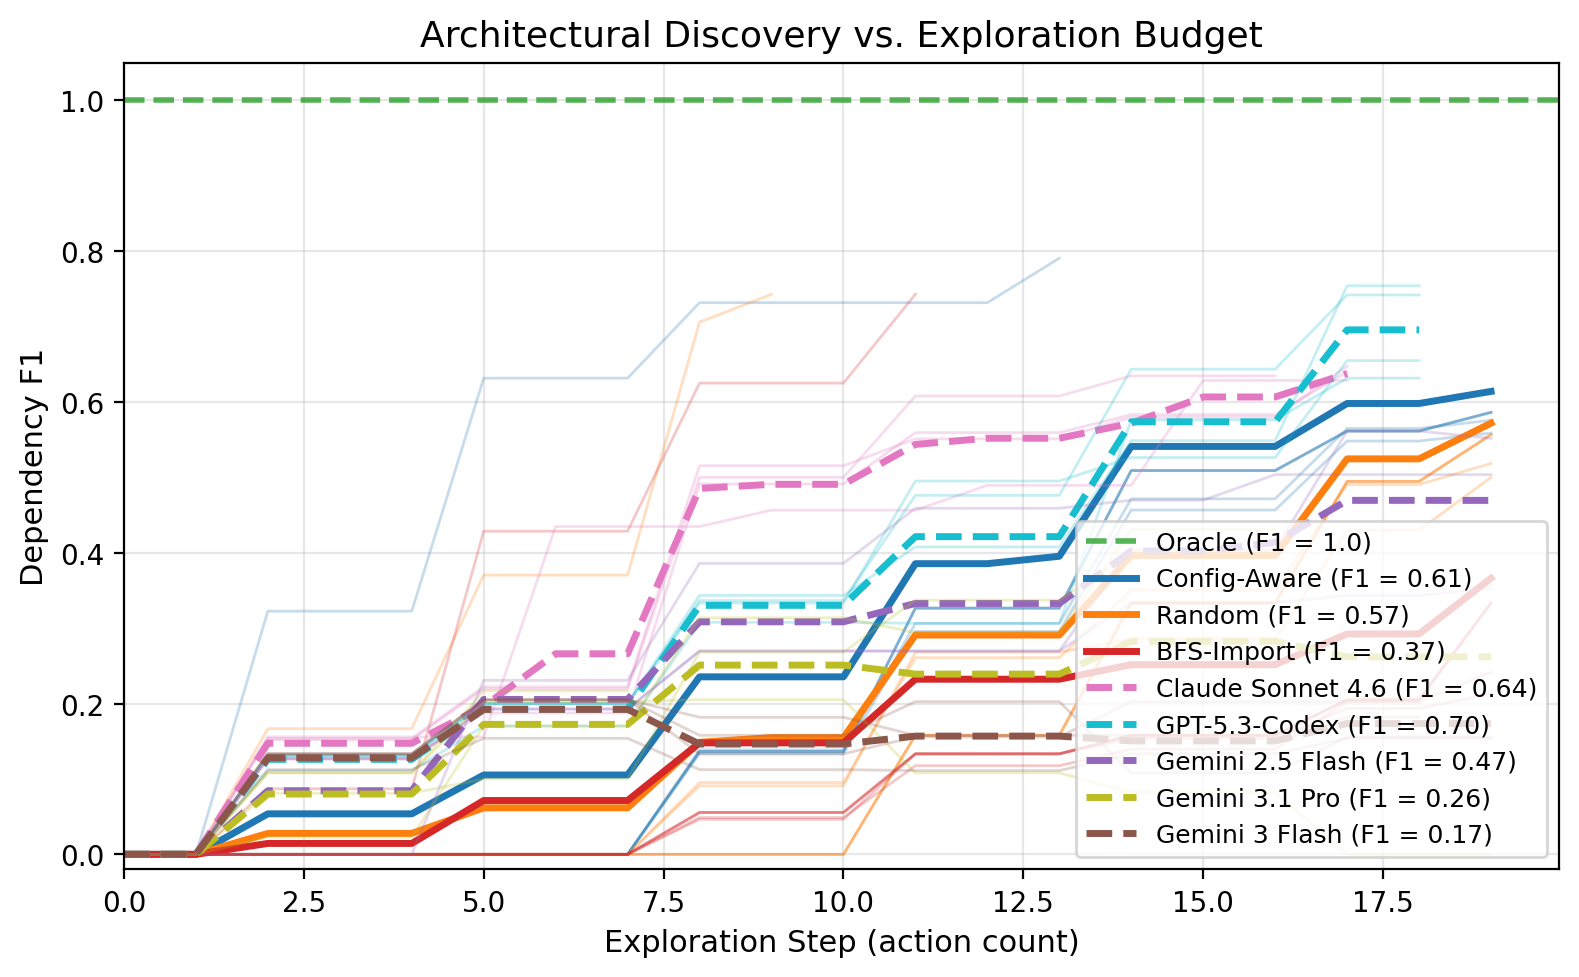
\includegraphics[width=\textwidth]{figures/f1_vs_steps.png}
        \caption{F1 vs.\ exploration steps. Dashed = LLM agents, solid = baselines. GPT-5.3-Codex reaches highest final F1; Claude Sonnet~4.6 leads on efficiency (AUC).}
        \label{fig:f1_steps}
    \end{subfigure}
    \hfill
    \begin{subfigure}[b]{0.48\textwidth}
        \centering
        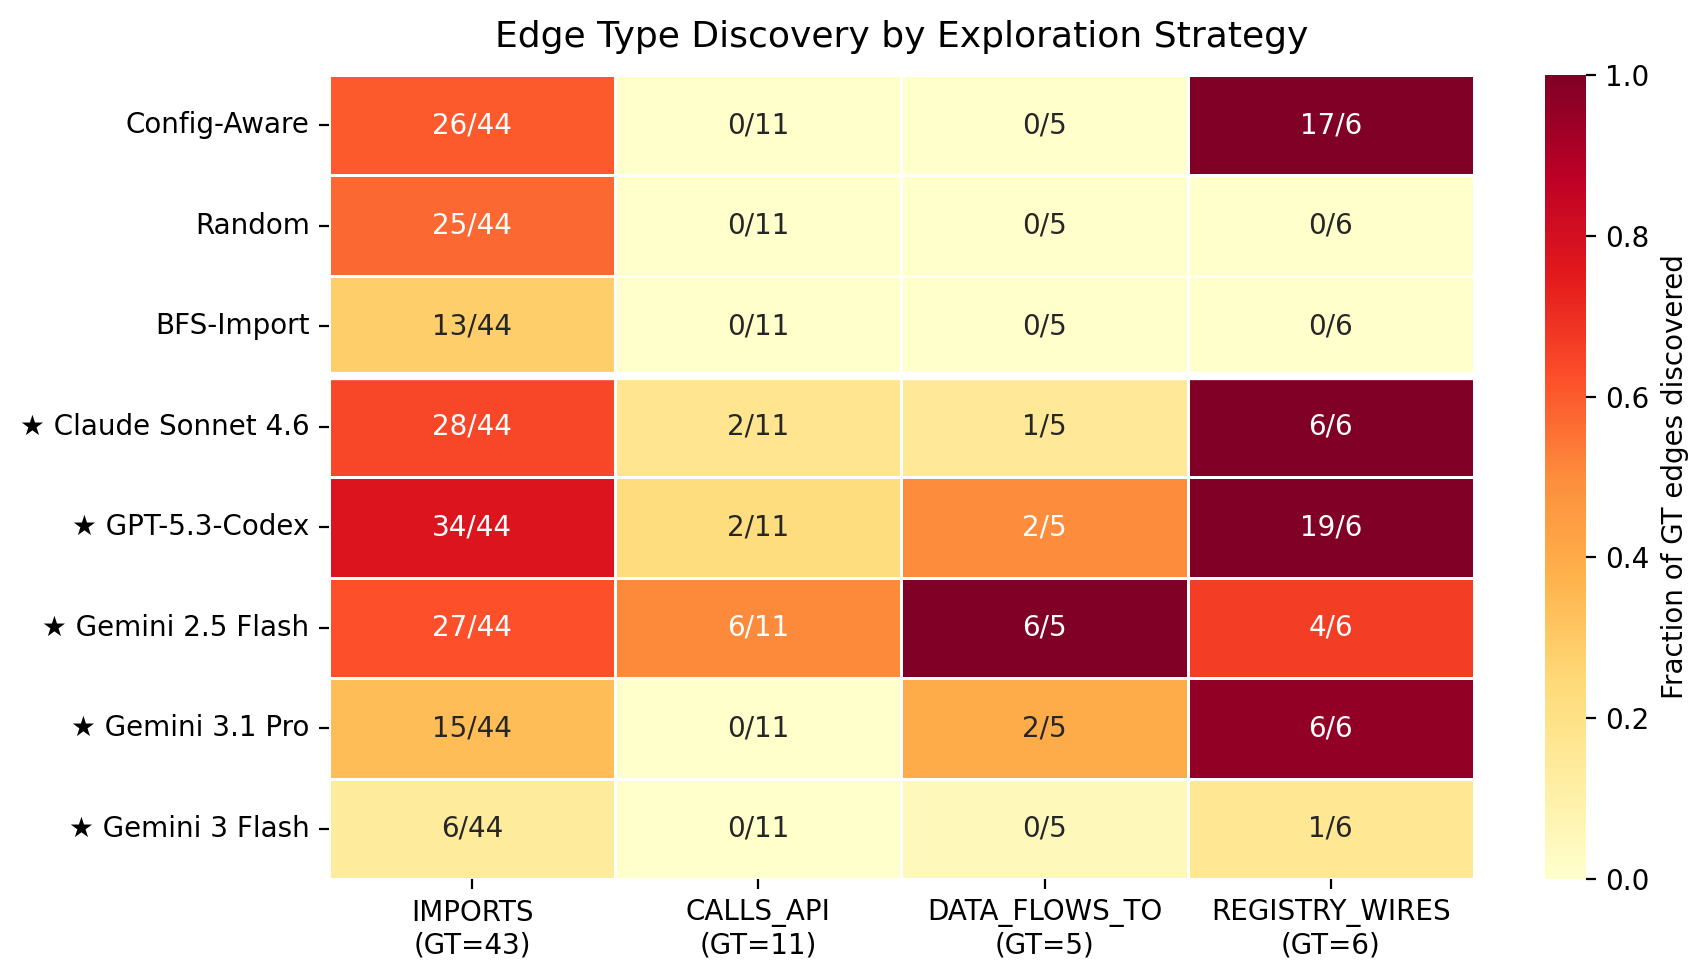
\includegraphics[width=\textwidth]{figures/edge_type_discovery.png}
        \caption{Edge type discovery heatmap. Cells show raw count / ground truth. LLM agents ($\star$) discover all four edge types; baselines find at most two.}
        \label{fig:edge_types}
    \end{subfigure}

    \vspace{0.5em}
    \begin{subfigure}[b]{0.70\textwidth}
        \centering
        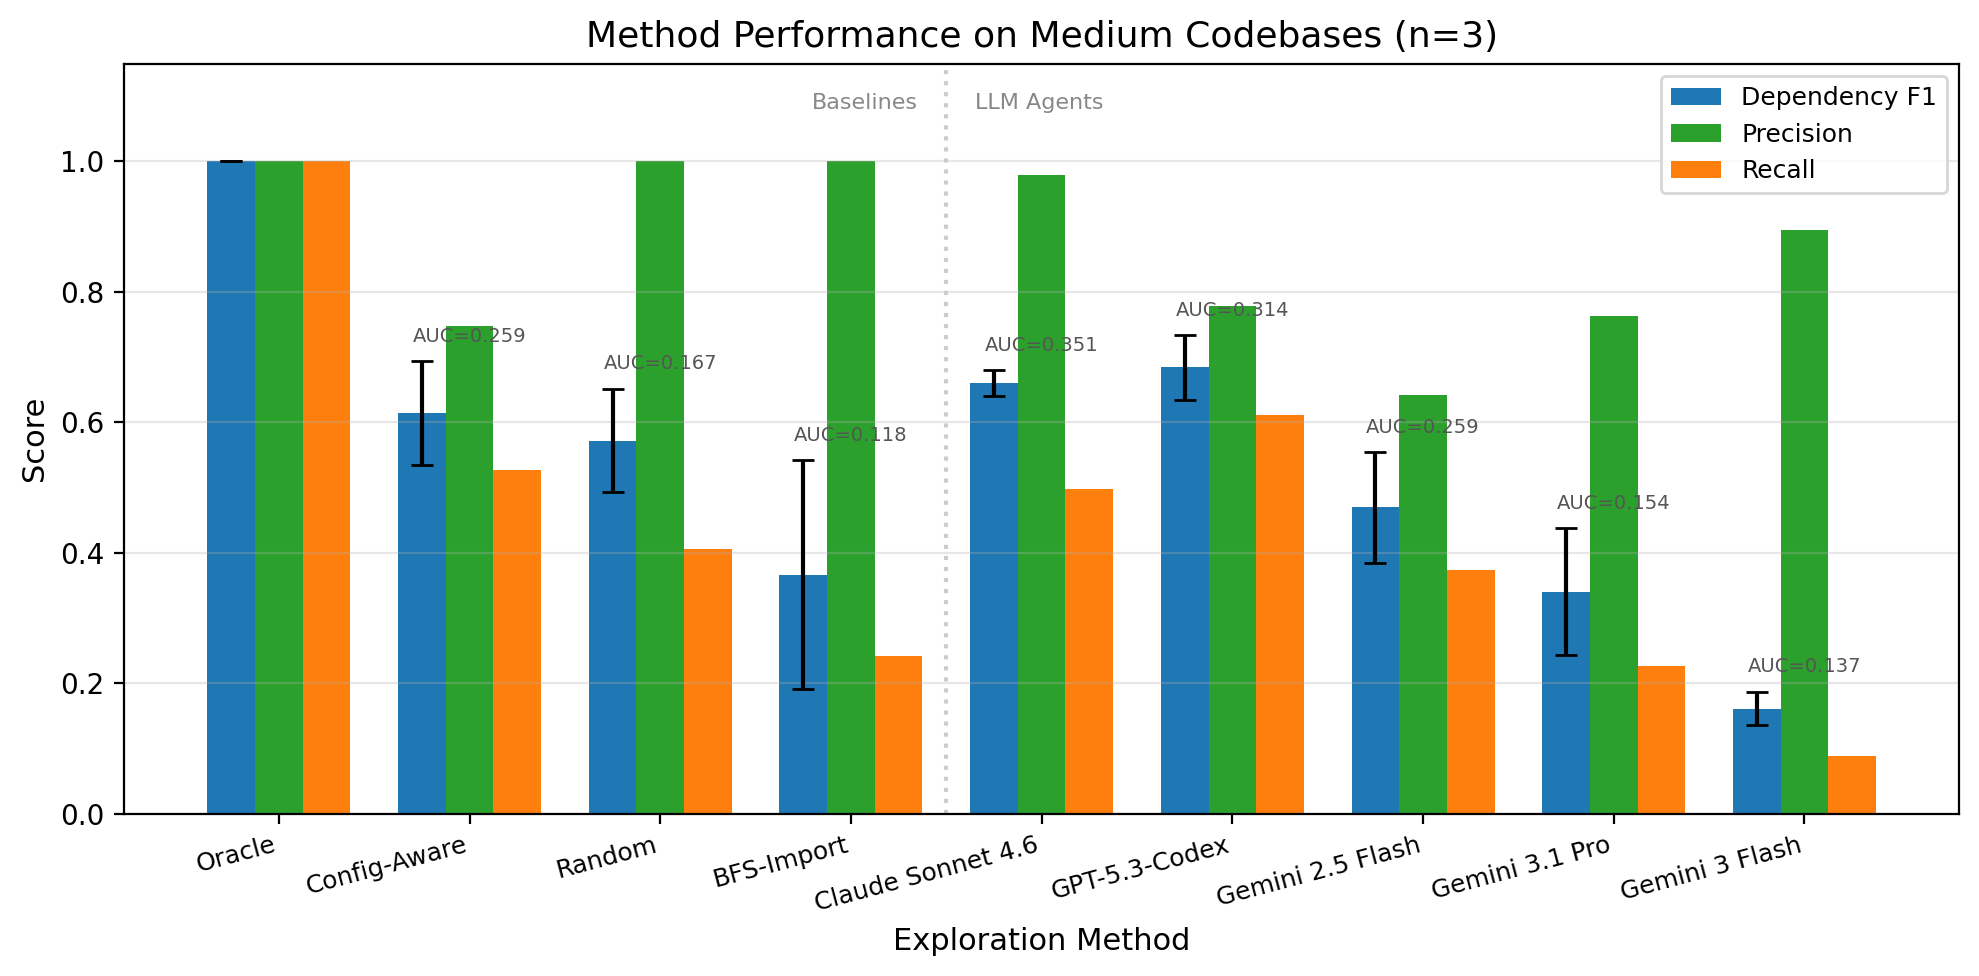
\includegraphics[width=\textwidth]{figures/baseline_comparison.png}
        \caption{Precision, recall, and F1 per method. GPT-5.3-Codex and Claude Sonnet~4.6 surpass all baselines; weaker LLMs show high precision but low recall.}
        \label{fig:bar_chart}
    \end{subfigure}
    \caption{Exploration analysis across 4 baselines and 6 LLM agents on medium-complexity codebases ($n{=}3$, budget $B{=}20$).}
    \label{fig:main}
\end{figure}

\subsection{Analysis}

The following observations are based on a single run per model-codebase pair across six LLM agents from three providers. We present them to illustrate the benchmark's discriminative power; the specific rankings and effect sizes should be treated as preliminary until confirmed with repeated runs and additional models.

\paragraph{Two LLM agents surpass all baselines.}
GPT-5.3-Codex achieves the highest Dependency F1~=~0.676, and Claude Sonnet~4.6 reaches F1~=~0.664, both surpassing the best rule-based strategy (Config-Aware, 0.577) by 9--10 points. GPT opens 15 files per codebase (vs.\ 13 for baselines) and attains the highest recall (0.597), while Claude opens only 13 files but with near-perfect precision (0.983). This precision-recall tradeoff reflects different exploration strategies: GPT favors broad coverage, Claude favors targeted, confident exploration. Both discover \emph{all} ground-truth REGISTRY\_WIRES edges (Table~\ref{tab:edge_types})---matching Config-Aware's recall but with GPT matching Config-Aware's 33\% precision on this type (over-generating false positives) while Claude achieves perfect REGISTRY\_WIRES precision (zero false positives).

\paragraph{LLM agents discover all four edge types.}
Table~\ref{tab:edge_types} reveals the most distinctive finding: \textbf{LLM agents collectively discover all four edge types}, while baselines find at most two (IMPORTS and REGISTRY\_WIRES for Config-Aware). GPT-5.3-Codex achieves the highest IMPORTS recall (69\%, exceeding even Config-Aware's 58\%). For DATA\_FLOWS\_TO edges---which require multi-hop reasoning, tracing one module's return value through the runner into the next module's input---Gemini~3.1~Pro achieves the highest recall (50\%), with perfect discovery on one codebase (6/6 inter-stage data flow edges), followed by GPT-5.3-Codex (31\%). Claude found zero DATA\_FLOWS\_TO edges despite reading the runner code---it inferred REGISTRY\_WIRES from the config alone without reading enough stages to trace data flow. This \emph{exploration-comprehension tradeoff} shows that even correct understanding of the orchestrator is insufficient---agents must also open the linked modules to infer inter-stage data dependencies. Gemini~2.5~Flash discovers CALLS\_API (18\% recall) and REGISTRY\_WIRES (37\% recall) edges invisible to BFS-Import and Random baselines.

\paragraph{Improved prompts unlock invariant discovery.}
With improved probe prompts providing per-type field semantics and pairwise decomposition instructions, LLM agents achieve substantial invariant F1 under relaxed matching (\S\ref{sec:probing}): Claude Sonnet~4.6 leads with 0.778, GPT-5.3-Codex achieves 0.739, and Gemini~2.5~Flash reaches 0.517. This is a dramatic improvement over the zero scores obtained with the earlier prompt version, confirming that invariant discovery was primarily a prompt specification problem rather than a model capability gap (\S\ref{sec:discussion}). Gemini~2.5~Pro achieves 0.376, while Gemini~3~Flash---which struggles with edge discovery---scores only 0.125. Baselines score zero on invariants as they cannot reason about cross-cutting constraints.

\paragraph{The belief externalization bottleneck.}
The three Gemini models illustrate the belief externalization problem with distinct failure modes. Gemini~2.5~Flash opens 14 files (comparable to baselines) and demonstrates clear code comprehension---action logs show import-chain-following behavior. Yet its IMPORTS recall (47\%) lags behind Config-Aware (58\%) and GPT (69\%) due to (1)~\emph{granularity mismatch}: reporting directory-level edges instead of file-level edges; and (2)~\emph{inference under-reach}: recognizing patterns but failing to report all visible imports. \textbf{Gemini~2.5~Pro and 3~Flash reveal a more fundamental failure: catastrophic belief state instability.} Despite opening comparable numbers of files, both models fail to \emph{accumulate} knowledge across probes. Gemini~3~Flash exhibits recency bias---each probe reports only 3--5 recently-examined components, discarding earlier discoveries entirely. Gemini~2.5~Pro shows a different pattern: it builds a reasonable map (peak F1~=~0.33 at step~9) then \emph{destroys} it, losing 12 correct edges in a single probe step. In contrast, Gemini~2.5~Flash loses zero correct edges across all probes---pure monotonic accumulation. This suggests that \textbf{belief state maintenance}---not just externalization format---is itself a non-trivial capability that varies dramatically across model versions. The gap between what an agent \emph{has seen} and what it \emph{retains in its belief state} is a first-order confounder in any belief-probing benchmark.

\paragraph{Precision-recall profiles differ qualitatively.}
Baselines using AST parsing (BFS-Import, Random) achieve perfect precision---every reported edge is correct. Among LLMs, Claude Sonnet~4.6 and Gemini~2.5~Pro both achieve near-perfect precision (0.983 and 1.000 respectively), but with dramatically different recall: Claude attains 0.502 while Gemini~2.5~Pro manages only 0.138. This decoupling reveals that high precision alone does not indicate strong architectural understanding---it may simply reflect extreme conservatism. GPT-5.3-Codex trades some precision (0.782) for the highest recall (0.597). Gemini~2.5~Flash has the lowest LLM precision (0.642), generating false CALLS\_API and DATA\_FLOWS\_TO edges alongside its correct discoveries.

\paragraph{Efficiency strongly favors LLM agents.}
Under the Action AUC metric---which rewards early discovery---Claude Sonnet~4.6 dominates (0.350), followed by GPT-5.3-Codex (0.306), both well above Config-Aware (0.212). Gemini~2.5~Flash (0.259) outperforms all baselines except Config-Aware on AUC, while Gemini~2.5~Pro (0.205) falls just below Config-Aware despite its perfect precision. This reflects the tradeoff between comprehension quality and externalization completeness: strong AUC requires both understanding \emph{and} reliably reporting that understanding at each probe point.

\paragraph{Random's competitiveness and budget effects.}
Random exploration (F1~=~0.538) performs nearly as well as Config-Aware (0.577). This near-parity reflects the current scale: budget $B{=}20$ on 27--30 modules allows opening roughly half the files, making raw coverage a strong proxy for import discovery. A budget sweep (Appendix~\ref{app:budget}) confirms that at $B{=}10$, Config-Aware's advantage grows to 3$\times$ over Random (0.175 vs.\ 0.056). The meaningful discrimination at $B{=}20$ lies in \emph{understanding what you've seen}: LLM agents discover qualitatively different edge types despite comparable file coverage.

% ============================================================================
\section{Discussion}
\label{sec:discussion}

\subsection{Implications for Code Agent Design}

Current code agents (SWE-agent, Aider, Claude Code, Cursor) use tool-augmented retrieval to navigate repositories, but none explicitly construct or maintain a structured architectural belief. Our results show that the strongest LLM agents \emph{can} surpass rule-based strategies when they combine semantic comprehension with reliable belief externalization (GPT-5.3-Codex and Claude Sonnet~4.6 both exceed all baselines), but that weaker models fail at the externalization step despite demonstrating code understanding in their exploration behavior.

This suggests four improvement paths: (1)~\textbf{hybrid approaches} combining AST-level import extraction with LLM semantic analysis, ensuring structural completeness while adding semantic depth; (2)~\textbf{belief externalization training}---explicitly optimizing models to faithfully serialize architectural knowledge into structured formats; (3)~\textbf{exploration strategy optimization}---broader file coverage (GPT's 15 files vs.\ Claude's 13) directly correlates with higher recall and unique edge type discovery; and (4)~\textbf{explicit state management}---providing agents with a persistent, accumulative data structure rather than relying on implicit belief state maintenance, which our results show can catastrophically fail even in capable models.

\subsection{The Belief Externalization Problem}

The spread across models is striking: GPT-5.3-Codex recalled 69\% of IMPORTS edges, while Gemini~3~Flash and Gemini~2.5~Pro recalled only 11--12\% despite opening a similar number of files. This 6$\times$ gap in IMPORTS recall---for edges the models demonstrably \emph{saw}---suggests that belief externalization capability varies dramatically across model families, not just between LLMs and baselines.

Both GPT-5.3-Codex and Claude Sonnet~4.6 demonstrate that faithful externalization \emph{is} achievable with current models: Claude with near-perfect precision (0.983), GPT with the highest recall (0.597). The challenge appears model-specific rather than fundamental: it is not that structured JSON is inherently difficult to produce, but that some models have not been optimized for this capability.

\paragraph{Belief state instability: a new failure mode.}
The Gemini model family reveals a striking failure mode beyond simple externalization weakness: \textbf{belief state instability} that manifests in three distinct patterns across four models. Gemini~2.5~Pro shows \emph{catastrophic collapse}: building a reasonable map by step~9 (peak F1~=~0.33), then losing 12 correct edges in a single probe step (F1~$\to$~0.09), before partially recovering. Gemini~3~Flash shows \emph{severe recency bias}: each probe reports only 3--5 recently-examined components with no accumulation. Gemini~3.1~Pro shows \emph{variable instability}: on its best codebase (F1~=~0.458) it accumulates monotonically like strong models, but on its worst (F1~=~0.203) it degrades to Gemini-3-Flash-level recency bias---the map collapses to zero edges at step~18 before partially recovering. This high variance (half-range $\pm$0.128) makes Gemini~3.1~Pro the least consistent model in our evaluation.

Critically, Gemini~2.5~Flash---the smallest model in the family---exhibits \textbf{zero} correct-edge loss across all probes, with purely monotonic accumulation. This counter-intuitive result (the smallest model maintaining the most stable beliefs) suggests that belief state maintenance is not simply a function of model scale but may depend on training objectives or architectural choices. The instability appears to stem from treating each probe as ``summarize the architecture from scratch'' rather than ``incrementally update your running belief state''---a fundamental misinterpretation of the task that prompt design alone may not resolve.

Importantly, externalization quality is likely \emph{prompt-dependent}: the same model may produce higher-quality maps under different prompt designs (e.g., few-shot examples, step-by-step decomposition, explicit schema walkthroughs, or chain-of-thought elicitation before the final JSON). Our use of identical prompts across all models controls for this variable experimentally but measures performance under a \emph{specific prompt regime} rather than each model's ceiling. Future work should include prompt ablation studies---varying schema detail, number of examples, and elicitation strategy---to disentangle model capability from prompt sensitivity.

\paragraph{Case study: prompt ambiguity and edge type confusion.}
Error analysis of Gemini~2.5~Flash's 40 false positive edges across 3 codebases reveals that \textbf{only 2 (5\%) are true hallucinations}---fabricated relationships with no basis in the code. The remaining 95\% reflect real relationships reported in the wrong format or with the wrong edge type. Crucially, many of these ``errors'' stem from \emph{ambiguity in the probe prompt itself}.

The dominant failure mode (45\% of FPs) is \emph{edge type confusion}: when the model sees \texttt{from config import PipelineConfig} followed by \texttt{PipelineConfig()}, it reports both an IMPORTS edge \emph{and} a CALLS\_API edge. Our probe defines CALLS\_API as ``the file calls a public function exported by the target,'' but does not state whether edge types are mutually exclusive, whether class instantiation counts as ``calling a function,'' or whether an edge should be IMPORTS or CALLS\_API when both an import statement and a function call exist. Gemini's interpretation---reporting both---is arguably reasonable given the underspecified definitions. Claude Sonnet~4.6 happens to match the ground-truth convention, but this may reflect better prompt compliance rather than deeper understanding:

\begin{center}
\small
\begin{tabular}{@{}lll@{}}
\toprule
\textbf{Edge} & \textbf{Gemini 2.5 Flash} & \textbf{Claude Sonnet 4.6} \\
\midrule
\texttt{cli $\to$ config} & IMPORTS & IMPORTS \\
\texttt{cli $\to$ runner} & IMPORTS & IMPORTS \\
\texttt{cli $\to$ config::PipelineConfig} & CALLS\_API {\color{red}(FP)} & --- \\
\texttt{cli $\to$ runner::run\_pipeline} & CALLS\_API {\color{red}(FP)} & --- \\
\texttt{cli $\to$ runner} & --- & CALLS\_API {\color{green!50!black}(TP)} \\
\bottomrule
\end{tabular}
\end{center}

\noindent Similarly, 22\% of FPs come from treating non-component files (tests, JSON configs) as edge endpoints---but the prompt does not explicitly define what counts as a ``component.'' This taxonomy reveals that \textbf{prompt specification is itself a first-order variable} in belief-probing benchmarks: what looks like an externalization failure may be a legitimate alternative interpretation of underspecified instructions. Future versions should provide explicit edge type decision rules (e.g., ``if both IMPORTS and CALLS\_API apply, report only CALLS\_API'') and an explicit component whitelist or exclusion criteria.

\subsection{Documentation as a Discovery Channel}

Real codebases contain rich documentation beyond code: README files, architecture decision records (ADRs), API specifications (OpenAPI/Swagger), and external resources (wikis, design documents). These serve as a major architectural discovery channel that our v0.1 codebases---which contain only code-level docstrings---do not yet model.

Extending the generator to produce standalone documentation files opens several directions. First, some architectural edges or invariants could be discoverable \emph{only} through documentation, testing whether agents read docs or dive straight into code. Second, documentation \emph{staleness}---a pervasive real-world problem where docs describe a prior version of the architecture---creates a natural testbed for the REVISE evaluation mode: agents would need to reconcile contradictions between documentation and code, deciding which to trust. Third, external documentation could be modeled as an additional action (e.g., \texttt{FETCH\_DOC}) with its own budget cost, testing whether agents know when to look outside the repository.

\subsection{Benchmark Design Lessons}

Building and running \tocs{} v0.1 exposed several pitfalls in belief-probing benchmark design that we document here for the benefit of future work.

\paragraph{L1: Define edge type semantics with decision rules, not just descriptions.}
Our probe prompt defines CALLS\_API as ``the file calls a public function exported by the target'' alongside IMPORTS as ``a Python import statement exists.'' When code both imports and calls a symbol, models must decide which edge type to report---but the prompt does not state whether types are mutually exclusive, nor whether class instantiation counts as ``calling a function.'' This ambiguity caused 45\% of Gemini~2.5~Flash's false positives (\S\ref{sec:discussion}). \emph{Fix:} provide explicit decision trees (e.g., ``if a file imports \emph{and} calls a symbol, report CALLS\_API only; report IMPORTS only for unused imports'').

\paragraph{L2: Define component boundaries explicitly.}
Our probe prompt asks models to list ``components'' but never defines whether test files, configuration files, or \texttt{\_\_init\_\_.py} files qualify. Models that included \texttt{test\_smoke.py} or \texttt{pipeline\_config.json} as edge endpoints were penalized despite identifying real relationships. \emph{Fix:} provide an explicit inclusion rule (e.g., ``components are Python source files excluding tests and configs'') or enumerate valid components in the probe.

\paragraph{L3: Specify structured field semantics per invariant type.}
Our initial invariant schema used generic fields (\texttt{src}, \texttt{dst}, \texttt{via}) without per-type semantics, and all models scored Invariant F1~=~0.0. After adding per-type field definitions and worked examples in the improved prompt, invariant F1 jumped to 0.52--0.78 under relaxed matching---confirming this was a prompt specification problem, not a model capability gap.

\paragraph{L4: Validate scoring against alternative correct answers.}
Strict exact-match scoring conflates format compliance with architectural understanding. A model reporting \texttt{registry.py $\to$ stages/} with 7 REGISTRY\_WIRES edges ``knows'' the same fact as the 7 file-level ground-truth edges but receives zero credit. \emph{Fix:} implement tiered scoring (full credit for exact match, partial credit for semantically equivalent answers) or normalize predictions before comparison.

\paragraph{L5: Prompt specification is a first-order experimental variable.}
Across all failure modes, the recurring theme is that \emph{what looks like a model capability gap may be a prompt specification gap}. We recommend that belief-probing benchmarks treat their probe prompts as artifacts requiring the same rigor as evaluation metrics---versioned, ablated, and reported alongside results.

\paragraph{L6: In scratchpad mode, probe prompts affect exploration, not just scoring.}
We ran all four LLM agents on the \emph{same three codebases} under two probe prompt versions: an initial version with minimal schema guidance, and an improved version adding per-type field semantics, file-path granularity instructions, and pairwise invariant decomposition examples. In our \texttt{probe\_as\_scratchpad} track, the agent's JSON map response is retained in its conversation context, serving as a self-assessment visible to the agent on subsequent turns. Table~\ref{tab:prompt_ablation} shows consistent F1 improvements across all models, but with dramatically different magnitudes.

\begin{table}[h]
\centering
\caption{Effect of improved probe prompt on Dependency F1 (same 3 codebases, same models, only probe prompt changed). $\Delta$ = new $-$ old.}
\label{tab:prompt_ablation}
\begin{tabular}{@{}lccc@{}}
\toprule
\textbf{Model} & \textbf{Old Prompt} & \textbf{New Prompt} & $\boldsymbol{\Delta}$\textbf{F1} \\
\midrule
Gemini 2.5 Flash & 0.328 & 0.469 & +0.141 \\
GPT-5.3-Codex & 0.564 & 0.676 & +0.113 \\
Claude Sonnet 4.6 & 0.639 & 0.650 & +0.012 \\
\bottomrule
\end{tabular}
\end{table}

The mechanism is \emph{not} just better serialization. Action log analysis reveals that in \texttt{probe\_as\_scratchpad} mode, the improved prompt changes exploration behavior itself. On one codebase (seed~999), GPT-5.3-Codex follows an \emph{identical} action sequence under both prompts for the first 15 steps; at step~16---immediately after a probe point---the old run opens a utility file and stops, while the new run opens 4 additional stage modules. The more structured probe revealed gaps in the agent's own map, causing it to redirect remaining budget toward coverage. This yielded 26 additional correct edges (F1 from 0.392 to 0.636 on that codebase alone). Claude Sonnet~4.6, which already externalized comprehensively under the old prompt, showed minimal improvement (+0.012)---suggesting its belief externalization was already near-ceiling. This has two implications for benchmark design: (1)~in scratchpad mode, the probe is not a passive measurement instrument but an \emph{active intervention} that shapes the agent's exploration policy; and (2)~models with weaker baseline externalization benefit disproportionately from prompt improvements, meaning model rankings are partially prompt-dependent.

\subsection{Limitations}

\tocs{} v0.1 is deliberately narrow in scope. Generated codebases, while structurally realistic, may not capture all patterns of real-world architecture. In particular, our use of neutral filenames (\texttt{mod\_a.py} rather than \texttt{authentication\_service.py}) removes naming priors that real codebases provide, making the task harder in one dimension while keeping it easier in others (clean structure, no organic complexity, limited dead code). This design choice isolates architectural reasoning from lexical guessing, but means our difficulty estimates may not transfer directly to real repositories. Additionally, our generated codebases contain only code-level documentation (docstrings) and lack standalone documentation files (README, ARCHITECTURE.md, design documents) that real repositories provide as a major architectural discovery channel. We evaluate a single architectural pattern (Pipeline) in a single language (Python). Our LLM results are preliminary: six models from three providers, each evaluated on 3 codebases with a single run per model-codebase pair (no variance estimation across runs). All LLM results use a single prompt design; different formulations could yield substantially different rankings. Our improved probe prompt addresses several ambiguities from the initial version (per-type field semantics, pairwise decomposition, edge type decision rules) and substantially improved invariant scores, but may still contain underspecifications. The cognitive map externalization is a proxy for internal representation---a model may ``know'' more than it serializes, as the wide variation across models suggests. We plan to expand to additional models (open-weight), architectural patterns, repeated runs with variance estimation, and the REVISE evaluation mode.

\subsection{Community Call}

We release the complete \tocs{} toolkit---codebase generator, partial observability harness, evaluation pipeline, and scoring metrics---as open-source software. We invite the community to:
\begin{enumerate}[nosep]
    \item \textbf{Evaluate additional models}: Run open-weight models (Llama, Qwen, DeepSeek) and replicate our frontier model results with repeated runs.
    \item \textbf{Contribute codebase patterns}: Extend beyond Pipeline to event-driven, microservices, plugin systems, hexagonal architecture (see CONTRIBUTING.md).
    \item \textbf{Add languages}: The harness is language-agnostic; the generator needs new templates for TypeScript, Go, etc.
    \item \textbf{Test scaffold-augmented agents}: Evaluate whether static analysis tools, RepoMap-style context, or explicit state tracking improve map quality.
\end{enumerate}

% ============================================================================
\section{Conclusion}
\label{sec:conclusion}

We introduced \tocs{}, a benchmark for evaluating whether code agents can construct coherent architectural beliefs through active codebase exploration under partial observability. Our procedural generator produces medium-complexity codebases with four typed edge categories and planted invariants. Preliminary experiments with four baselines and six frontier LLM agents from three providers reveal that: (1)~the two strongest LLM agents (GPT-5.3-Codex, F1~=~0.676; Claude Sonnet~4.6, F1~=~0.664) surpass all baselines by combining semantic comprehension with reliable belief externalization; (2)~LLM agents collectively discover all four edge types---including DATA\_FLOWS\_TO edges (Gemini~3.1~Pro, 50\% recall; GPT-5.3-Codex, 31\%) and REGISTRY\_WIRES edges (GPT and Claude, 100\% recall)---capabilities entirely absent from rule-based methods; (3)~improved probe prompts unlock invariant discovery (relaxed F1 up to 0.78), confirming that invariant scoring failures were primarily a prompt specification problem; yet (4)~weaker LLM agents score below simple heuristics due to catastrophic belief state instability---some models lose previously-discovered edges between probes, with a 6$\times$ spread in IMPORTS recall across models (11--69\%), confirming that both belief externalization and belief state maintenance remain key capability gaps. The 32-point F1 gap between Oracle and the best LLM agent defines a challenging and discriminative evaluation space. We release \tocs{} as an open benchmark and invite the community to replicate and extend these preliminary results.

% ============================================================================
\bibliographystyle{plainnat}
\bibliography{references}

% ============================================================================
\appendix

\section{Evaluation Prompts}
\label{app:prompts}

\paragraph{System prompt (excerpt).} The agent is told: ``You are an expert software engineer exploring a codebase you have never seen before. You are operating under PARTIAL OBSERVABILITY [...]  Available actions: LIST, OPEN, SEARCH, INSPECT, DONE. [...] Your goal is to build a complete and accurate ARCHITECTURAL UNDERSTANDING.'' The full prompt describes action semantics and exploration strategy tips.

\paragraph{Cognitive map probe.} After every $K$ actions, the agent receives: ``Externalize your current architectural belief as JSON matching the following schema [...]'' The schema specifies components with status/purpose/exports/edges/confidence, invariants with structured canonical form, and an uncertainty summary. A worked example demonstrates the expected format (see supplementary materials).

\section{Generated Codebase Example}
\label{app:example}

A medium-complexity codebase (seed 42, text processing domain) generates the following structure:
\begin{verbatim}
text_processor/
+-- __init__.py          +-- middleware/
+-- models.py            |   +-- mod_i.py (logging)
+-- base.py              |   +-- mod_j.py (retry)
+-- config.py            +-- utils/
+-- exceptions.py        |   +-- helpers.py
+-- registry.py          |   +-- formatters.py
+-- stages/              +-- legacy/
|   +-- mod_a.py         |   +-- old_pipeline.py
|   +-- mod_b.py         |   +-- compat.py
|   +-- mod_c.py         +-- runner.py
|   +-- mod_d.py         +-- cli.py
|   +-- mod_e.py         +-- pipeline_config.json
|   +-- mod_f.py         +-- test_smoke.py
+-- adapters/
|   +-- mod_g.py
|   +-- mod_h.py
\end{verbatim}

Stages implement a \texttt{StageBase} ABC. The registry loads stage ordering from \texttt{pipeline\_config.json}. Stages cannot import each other directly (enforced by test). Legacy modules are distractors not in the pipeline flow.

\section{Budget Sweep}
\label{app:budget}

To characterize how exploration budget affects discrimination between strategies, we ran all four baselines at $B \in \{10, 15, 20, 25\}$ across 3 codebases. Table~\ref{tab:budget} reports mean Dependency F1.

\begin{table}[h]
\centering
\caption{Dependency F1 vs.\ exploration budget (mean over 3 codebases).}
\label{tab:budget}
\begin{tabular}{@{}lcccc@{}}
\toprule
\textbf{Method} & $B{=}10$ & $B{=}15$ & $B{=}20$ & $B{=}25$ \\
\midrule
Oracle       & 1.000 & 1.000 & 1.000 & 1.000 \\
Config-Aware & 0.175 & 0.492 & 0.577 & 0.626 \\
Random       & 0.056 & 0.317 & 0.538 & 0.632 \\
BFS-Import   & 0.078 & 0.157 & 0.293 & 0.603 \\
\bottomrule
\end{tabular}
\end{table}

At tight budgets ($B{=}10$), Config-Aware's strategy of prioritizing registry files yields a 3$\times$ advantage over Random (0.175 vs.\ 0.056). As budget increases, raw coverage dominates: at $B{=}25$ (allowing agents to open nearly all files), Random matches Config-Aware (0.632 vs.\ 0.626). BFS-Import shows the steepest growth from $B{=}20$ to $B{=}25$ (0.293 $\to$ 0.603), reflecting its systematic but slow import-chain traversal. The convergence at high budgets confirms that the current medium-complexity codebases require \emph{tighter budgets} or \emph{larger codebases} to strongly discriminate exploration strategy for structural edge types; the meaningful discrimination at $B{=}20$ lies in semantic edge discovery by LLM agents.

\end{document}
